\documentclass[master,oneside,en,oldtitlepage]{dyplompwr}
\usepackage[utf8]{inputenc}
\usepackage[T1]{fontenc}

\usepackage{graphicx}
\usepackage{epstopdf}  %in Linux based system install texlive-font-utils to start using eps files
\epstopdfsetup{update}

\usepackage{hyperref}

% ==================== Packages ====================
% \usepackage[left=3cm, right=3cm, top=3cm, bottom=3cm]{geometry}   % Page margins
                                                                    % you can use showframe in geometry package to see the margins
                                                                
\usepackage{geometry}                   % For page margins and such
\usepackage{cite} 					            % For handling references
\usepackage{hyperref} 				          % For clickable links and references
\usepackage{xcolor}     			          % For text colors
\usepackage{indentfirst} 			          % Indent the first paragraph of a section
\usepackage[printonlyused]{acronym}     % For acronyms
\usepackage{amsmath}				            % For math equations
\usepackage{titlesec}				            % For customizing section titles
\usepackage[section]{placeins} 		      % For forcing figures to be in the same section
\usepackage[T1]{fontenc} 			          % For better font encoding
\usepackage{subcaption}				          % For subfigures
\usepackage{appendix}                   % For appendices
\usepackage{epstopdf}                   % For converting eps to pdf
\usepackage{adjustbox}                  % For adjusting the size of the images
\usepackage{pdflscape}                  % For landscape Packages
\usepackage{listings}
% =================== End Packages ===================
\newcommand{\todo}[1]{\textcolor{red}{\textbf{TODO: #1}}}
\lstset{
    basicstyle=\ttfamily\small,
    keywordstyle=\color{blue},
    stringstyle=\color{red},
    commentstyle=\color{green!50!black},
    numbers=left,
    numberstyle=\tiny\color{gray},
    frame=single,
    breaklines=true
}
% ==================== Settings ====================
% Customizing section titles
% Customizing section titles - modified for PWr template
% Optional customization
\titleformat{\chapter}[display]
  {\normalfont\huge\bfseries}{\chaptertitlename\ \thechapter}{20pt}{\Huge}
\titleformat{\section}
  {\normalfont\Large\bfseries}{\thesection}{1em}{}
\titleformat{\subsection}
  {\normalfont\large\bfseries}{\thesubsection}{1em}{}
\titleformat{\subsubsection}
  {\normalfont\normalsize\bfseries}{\thesubsubsection}{1em}{}
\titleformat{\paragraph}
  {\normalfont\normalsize\bfseries}{\theparagraph}{1em}{}

\setcounter{secnumdepth}{4}
\setcounter{tocdepth}{4}
\titleformat{\paragraph}
{\normalfont\normalsize\bfseries}{\theparagraph}{1em}{}
\titlespacing*{\paragraph}
{0pt}{3.25ex plus 1ex minus .2ex}{1.5ex plus .2ex}

% Set the path to the image folder
\graphicspath{
    {./images/}
}

% Line spacing can be adjusted here if needed
% \renewcommand{\baselinestretch}{1.5} 
% =================== End Settings ===================


% Input info here for the title page
\faculty{Faculty of Electronics, Photonics and Microsystems}
\fieldofstudy{Electronics}
\speciality{Advanced Applied Electronics}
\title{Design and analysis of free-space optical data link using SFP modules}
\author{Kacper Ugorny}
\supervisor{dr inż. Aleksander Głuszek}
\city{WROCŁAW}
\year{2026}

%Start of the document
\begin{document}

%Make title page
\maketitle
\setcounter{page}{2}

% Blank page according to template
\newpage
\null

% Page for abstracts
\newpage
\thispagestyle{plain}

\noindent\begin{minipage}[t][0.48\textheight][t]{\textwidth}
\noindent{\fontsize{20pt}{22pt}\selectfont\bfseries Streszczenie}

\vspace{8pt}
{\fontsize{16pt}{18pt}\selectfont
\setlength{\parindent}{1.5em}
\indent Polish abstract goes here.
}
\end{minipage}

\vspace*{0.04\textheight}

\noindent\begin{minipage}[t][0.48\textheight][t]{\textwidth}
\noindent{\fontsize{20pt}{22pt}\selectfont\bfseries Abstract}

\vspace{8pt}
{\fontsize{16pt}{18pt}\selectfont
\setlength{\parindent}{1.5em}
\indent English abstract goes here.
}
\end{minipage}

\newpage



\clearpage
\thispagestyle{empty}
\vspace*{0.5\textheight}
\begin{center}
    \it{Acknowledgements go here.}
\end{center}
\clearpage

\newpage

% Table of contents
\tableofcontents

% ============= Begin Acronyms ==================
\chapter{List of Acronyms}
\begin{acronym}[FOUR]\itemsep=-5pt
    \acro{FSO}{Free space optics}
    \acro{RF}{Radio frequency}
    \acro{ISM}{Industrial, Scientific, Medical Band - Free to use}
    \acro{DDM}{Digital Diagnostic Monitoring}
    \acro{OOK}{On Off Keying}
    \acro{NRZ}{Non-Return-To-Zero}
    \acro{RZ}{Return-to-Zero}
    \acro{LOS}{Line Of Sight}
    \acro{SFP}{Small Form-factor Pluggable}
    
\end{acronym}
% ============= End Acronyms ==================

% Main Text Block


\chapter{Introduction}
% This chapter sets the stage, explaining why your project matters and what you intend to achieve.
In a time of rapid global digitalization and great increase of need to process data, demand for high throughput and reliable communication systems keeps growing.
With the expand of data rates, the need for security also rises. 
Classic \ac{RF} systems, although widely used, might not satisfy needs of all customers, due to high traffic on unlicensed \ac{ISM} bands and possible unauthorized listening.

\ac{FSO} communication might meet the requirments that RF lacks and collect the most demanding users. 
Using precisly focused light beam, this solution not only exceeds RF solutions in terms of throughput, but also provides great security, by high directivity and difficulty of hijacking the signal.

Those characteristics makes the FSO systems highly competitive answer for need of private high throughput connections.
\section{Background}
% Brief introduction to Free Space Optical (FSO) communication and its advantages (high speed, license-free).
%Free space optical communication bases on transmitting data through the air using light source, typically a laser, which is detected on the other end by the photodiode.
%Such communication have planty of advantages, such as high data rates, license-free operation, and immunity to electromagnetic interference. 
%A very important aspect of FSO communication is security of such connection, because the beam is narrow and tapping into it breaks the connection.
%However, it also has some disadvantages, such as sensitivity to atmospheric conditions and the need for precise alignment.

Fundamental requirement of well functioning free space optical link is maintaining uninterrupted direct line of sight, between transmitter and receiver.
RF systems on the other hand diverge and bounce of the obstacles or even pass through them and still can reach the destination.
Ideally FSO systems, keep the transmitted beam collimated, what allows to achieve high power density and security of transmission at the expense of need for keeping precise alignment.
In practical deployments it is a challenging task because of environmental factors, such like vibrations, thermal expansion or atmospheric conditions.
That's why modern FSO systems are required to run advanced tracking and compensating systems.


\section{Motivation}
Although FSO systems are well described in scientific papers, developing such device is quite complex engineering task.
Main motivation of taking this topic is a need of creation affordable and functional proof of concept transcevier and establish a high throughput link. 
Completing such connection is challenging, because it requires knowledge of multiple fields: designing optical system, precise mechanics, electronics and low level embedded system programming with real time requirements.   

\section{Thesis Objectives}
%Clearly state your goal to design and develop a stable, high-speed FSO Ethernet link with active misalignment compensation.
Goal of this thesis is to design and develop a stable, affordable, high-speed FSO Ethernet link with active misalignment compensation.
This will be achieved by using low-cost, readily available SFP modules and a custom-built mechanical system for beam steering, controlled by a microcontroller that reads the \ac{DDM} data from the SFP module to maintain optimal alignment.
Realization of this link will be used as a platform to analyze practical issues induced by environmental factors. 
\section{Scope and Structure}
%A brief roadmap of the thesis document.
The rest of the document will provide information and knowledge about the theoretical background of FSO communication, the design and architecture of the system, the control algorithm used for active alignment, the experimental methodology, and finally the results and analysis of the project.
At the end conclusions will be drawn, it will be stated what wasn't optimal in taken solution and what should be done to improve a solution.



\chapter{Theoretical Background and State of the Art}
% Before showing your work, you need to prove you understand the physics and existing technology.
As it was stated in introduction, the task of creating a transcevier and then establishing the link is quite challenging, because of involvement of multiple scientific fields, such as:
precise mechanics, optics systems, electronics, motor control and low level firmware developing.
This chapter will showcase how such systems are working to give a reader breif understanding of issues that need to be overcome later in the development.


\section{Principles of FSO Communication}
%How optical data links work and their general architecture.
Generally, an FSO link is an set of two components: a transmitter and a receiver. 
The transmitter sends data signal in free space using modulated optical radiation. 
It consists of radiating element, which is usually a laser diode, a laser modulater and set of optics responsible for creating a beam.

Modulation is an essential functionaly in an optical transmitter. 
It allows for embedding data into light beam, which then travels the significant distance to the recevier.
Easiest way of modulating a optical signal is using direct modulation - changing an injection current of a laser diode, what affects the output optical power. 
That way on-off binary modulation can be achieved, more widely known as \ac{OOK}\cite{hui2025introduction}.
OOK simply trun on the light source to transmit a logic "one" and turns it off to transmit a "zero". 
There are two types of OOK which are \ac{NRZ} and \ac{RZ}. 
As a names suggest a RZ totally turns off the transmitter and a NRZ goes down to some level of output power.
RZ has advantage of higher sensitivity\cite{henniger2010introduction}.

Modulated light beam now enters an optical system that often consists of telescope or a collimator make the light beam capable of traveling long distances.
Such signal needs to travel through a open space to the receiver.
Line of sight of the transmitter and the receiver is required.
There are many factors that influence the path of the light, some directly like weather conditions and other indirectly like vibrations, wind or thermal expansion.
Taking those into consideration, tracking systems must be applied\cite{bloom2002physics}.

When the beam reaches it's destination, it enters the optic systems, which focuses it at the photodiode, which converts light into electrical signal.
Then demodulation of signal is done and data is received on the other end of the link.

\begin{figure}[htbp]
    \centering
    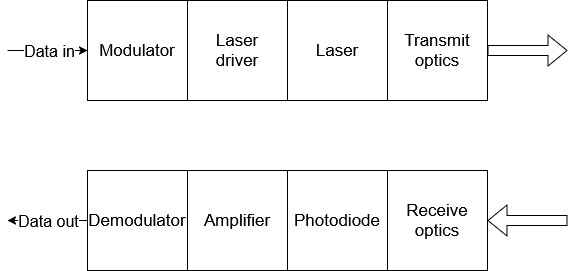
\includegraphics[width=0.8\textwidth]{figures/Simple_fso_diagram.jpg}
    \caption[short]{Example FSO system}
    \label{fig1:scheme}
\end{figure}






\section{Light Propagation and Environmental Factors}
Creation and development of FSO systems requires extensive knowledge about light propagation as well as awareness of things that affect the transmission.
Few of the examples are described below\cite{malik2015free}:
\begin{itemize}
  \item  Physical obstruction can temporally block the \ac{LOS}. For example a bird or a leaf might fly through the path.
  \item Absorption is coused by the molecules of the water, that occurs in the atmosphere. 
  Water dramatically decrease power of light passing through it.
  Especially fog is most limiting factor.
  \item Atmospheric turbulence might affect the beam, while passing through packets of air with different temperature therefore different refractive index.
  \item Atmospheric attenuation is a general factor which is a collection of different aspects like enironmental conditions - humidity or amount of dust in the air.
\end{itemize}

\section{SFP Modules and Digital Diagnostic Monitoring (DDM)}
A \ac{SFP} modules are standard peice of equipment that can be bought for affordable price. 
These are compact transceivers used in telecommunication.
SFP's plugged into a switch or a media converter convert electrical ethernet signal into modulated optical signal. 

It is intended to use them in fiber cable exceeding tens or even hundreds of kilometers.
SFP modules have different type of connectors, like RJ45 for electrical, LC and SC for optical. 
As written before these modules are transceivers, allowing for full duplex communication. 
It is realized by two physical optic channels or one optic channel using two different wavelenghts (eg. 1550nm Rx/1310nm Tx).

Typically SFP uses wavelenghts of telecommunication windows, which are 1st window - 850nm, 2nd window - 1310nm and 3rd window 1550nm. 
These wavelenghts are great for fiber communication because of low transmission loss in fibers.

SFP modules are implementing \ac{DDM}, which is management technology which lets users to monitor in real time few parameters of the transmission.
Those parameters are: output optical power, received power, temperature, laser current and transceiver supply voltage.

Mentioned characteristics makes a SFP modules great candidate for base element of FSO transcevier.
It drives the laser, handles the modulation and also implement the receving part.
Different connectors and wavelenghts configurations allows for different designs of the transceiver. 
DDM allows for real time data harvest, which is essential for tracking system.


\section{Existing Beam Steering Techniques}
FSO link during it existance, might destabilize, what can lead to loss of received power, reduction of throughput and in the worst case total loss of connection.
To limit the impact of environmental factors destroying the connection, providers of FSO links are implementing beam steering into their links.
On top of that aligment of long range link, without any beam steering is a tedious task.
At first glance it seems to be unnecessary, because in lab conditions link might work correctly, but deployment of long range link is a hard reality check.

The easiest way of providing beam steering into the design is to create a mechanical structure capable of rotating the whole transciver. 
Using such mechanism can provide big coverage and it is great solution when transceviers are placed on mobile platforms for example UAV drone.

Next possible solution is implementing translation into the optical system.
Movement of the lens or the mirror used to launch the beam, allows for change of angle in which the beam exits the transcevier.

Lastly the translation of optical element could be swapped with a tilt of the lens or the mirror, but tilting might introduce a increased level of difficulty, of understanding and modeling such movement.


\chapter{System Architecture and Hardware Design}
% This covers the [ENGINEERING ASPECT] of your thesis. It details the physical things you built.
This chapter will show and explain taken engineering choices used while building a FSO link which this document is all about.
It will start with general overview of the transceviers and the system in which such devices are deployable.
Next the mechanical and optical design will be shown and explained.
At the end the electronic circuit design will be showcased.

\section{Transcevier and Link Overview}
Transcievier architecture was carefuly chosen, to be realistic to finish in given deadline and also to be competitive on the market.
Another constraint was the affordability and availability of the elements on the market. Main elements which it consist of are:
\begin{itemize}
  \item gigabit SFP media converter,
  \item full duplex, 1.25GB/s, 80km, WDM, SFP 1490/1550 (rx/tx or tx/rx depending on the unit) SM SC connector providing one optical path, with DDM,
  \item 3d mechanical movement allowing for SFP translation,
  \item Nema 17 1.8 $\deg$ per step
  \item plano convex lens 50mm diameter, 85mm focal length.
  \item electical control system for driving the motors and tapping into SFP's DDM,
  \item esp32c6, for low throughput RF transmission,
\end{itemize}
  
\begin{figure}[htbp]
    \centering
    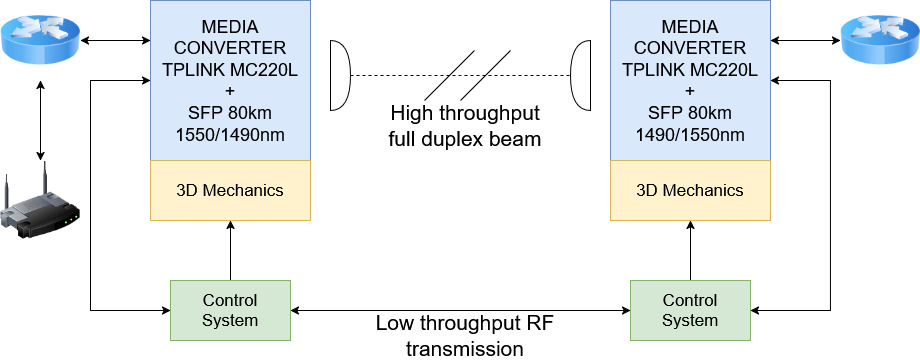
\includegraphics[width=.95\textwidth]{figures/System_diagram.jpg}
    \caption[short]{Transcevier and System diagram}
    \label{fig2:diag}
\end{figure}

\section{Mechanical and Optical Design}
%Details of the 3D-printed structure, lens positioning, and the integration of stepper motors for pan/tilt or lens shifting.
Crucial part of transcevier part is optical and mechanical design. 
In this particular case it is embedded together and movement provided by mechanics change the position of the light source to the lens.
It changes the angle in which light exists the transcevier, allowing for beam steering as showcased on \ref{fig3:Opt_exp}.

\begin{figure}[htbp]
    \centering
    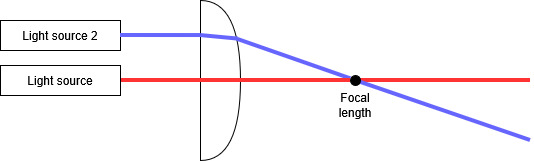
\includegraphics[width=1\textwidth]{figures/Optics_explanation.jpg}
    \caption[short]{Translation of light soruce against the lens}
    \label{fig3:Opt_exp}
\end{figure}

In case, when light source is placed in the focal length - the light beam will be collimated. 
Approximately if we move it in parallel to the lens the beam will be almost collimated and will exit the lens at the angle.
If there is second light beam coming into the transcevier at the same angle as the exiting beam, it will focus in same place as the light source is.
Thanks to this characteristic, this beam steering technique can work, allowing for transceviers to communicate when they are shifting from ideal alligment as shown at \ref{fig4:2_lenses}.

\begin{figure}[htbp]
    \centering
    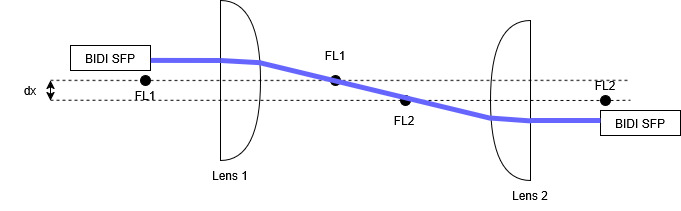
\includegraphics[width=1\textwidth]{figures/Lens_system1.jpg}
    \caption[short]{System of 2 transceviers}
    \label{fig4:2_lenses}
\end{figure}

To achieve such beam steering, proper mechanical system has been created, that allows for 3 axis movement of SFP module.
First axis, let's call it x is perpendicular to the lens and translation alongside this axis change the distance from SFP to the lens.
Another two axes, y and z are parallel to the lens and the moving the source in those direction steers the beam, as shown in the figure \ref{fig5:axes}. 

\begin{figure}[htbp]
    \centering
    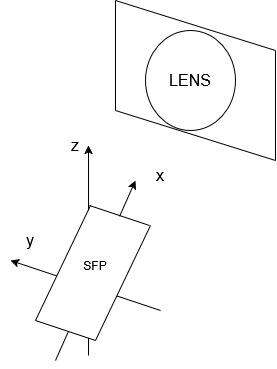
\includegraphics[width=0.4\textwidth]{figures/axis.jpg}
    \caption[short]{axes}
    \label{fig5:axes}
\end{figure}

Mechanical structure allowing movements alongside those axes has been based on lead screws and anti-backlash nut's rotated by stepper motors.
Used screw has 1 mm pitch, what means that one full rotation of the screw will move the element by 1 mm.
Beside lead screw, nuts and the bearings, rest of the mechanics was design for 3D printing.
While 3D printing dosen't give best proporties of the mechanical structure (Low stiffnes, thermal properties), it is great for rapid development and prototyping.

The 3D printed sturcture also includes a guides that elements move on. 
The shape of those guides in all axes was trapezoidal shape, as it can be seen in the figure \ref{fig6:Guides}.
At the right side there is shown hole which fits the guide rails. 
There are circles put in the corners in order to elimnate jamming of the sharp corners.

\begin{figure}[htbp]
    \centering
    \begin{minipage}{0.45\textwidth}
        \centering
        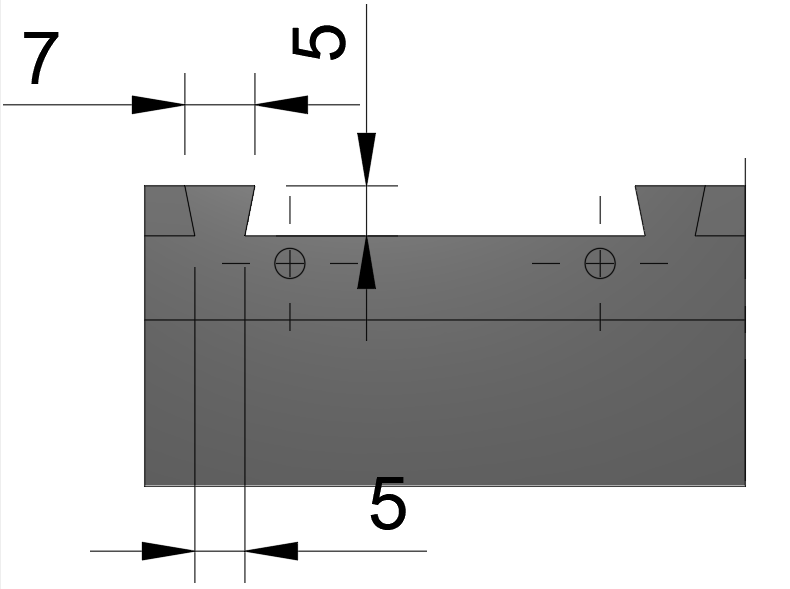
\includegraphics[width=\textwidth]{figures/X_Y_1.png} % Replace with your first image file
    \end{minipage}\hfill
    \begin{minipage}{0.45\textwidth}
        \centering
        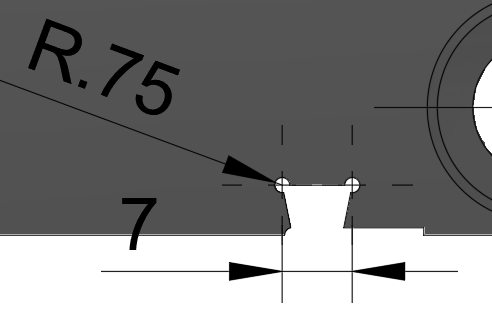
\includegraphics[width=\textwidth]{figures/X_Y_2.png} % Replace with your second image file
    \end{minipage}
    \caption{Left: Guide dimensions. Right: Guide hole}
    \label{fig6:Guides}
\end{figure}

\newpage
Mechanical movement was limited to 10mm x 10mm range of movement parallel to the lens by end switches.
Such range gives quite big range of motion, so it made a low range tests a bit easier.
Final structure is shown in the figure \ref{Fig7:Final}. 
As it can be noticed the whole sturcture is placed on the tripod, by custom made mount and there is mechanical "Iron sights" for ease of setting up the link.

\todo{DO nice photo of the whole transceiver}
\begin{figure}[htbp]
  \centering
  \includegraphics[width=0.7\textwidth]{figures/Final_structure.jpg}
  \caption[short]{Final transcevier}
  \label{Fig7:Final}
\end{figure}


\newpage
\section{Controller Design}
%The hardware required to run the system. Include your microcontroller choice, motor drivers, power supply, and the physical interface designed to read data from the SFP module.
A controller is a important part of the project, as it's running the whole transcevier. 
It consists of couple elements connected by GPIO's or communication protocols.
\begin{itemize}
  \item the heart of the controller is STM32F1 microcontroller,
  \item it's outputs are connected to the motor controllers A4988, which are configurated for 4 x microstepping,
  \item inputs are used to connect the end switches connected in series, so if any of the switches of the given axes are closed then it goes to one pin,
  \item I2C bus is used to connect the microcontroller to the SFP module, to hijack out the DDM data,
  \item There is also UART connection to the ESP32 microcontroller with PCB antenna serving as RF transceiver for communication in the link.
\end{itemize}

\begin{figure}[htbp]
  \centering
  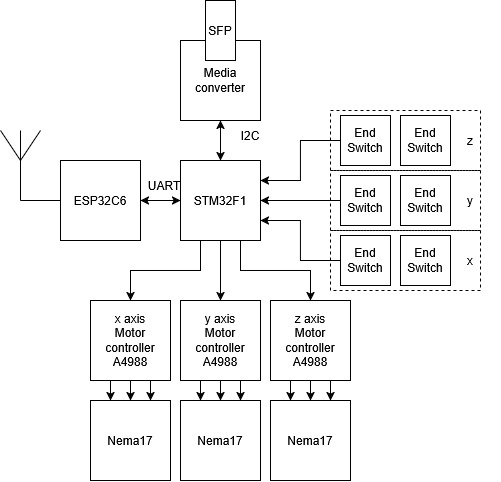
\includegraphics[width=0.85\textwidth]{figures/Electrical_scheme.jpg}
  \caption[short]{Block scheme of the controller}
  \label{Fig8:Controller}
\end{figure}
\newpage
The firmware, that is ran by the STM32 microcontroller, is a Non-Preemptive, 
Polling-Driven Single-Tasking Architecture, that calls multiple Finite State Machines (FSM).
Tasks that it runs are:
\begin{itemize}
  \item Movement Handler - it drives the motors and checks the end switches,
  \item Spiral Search FSM - controls the spiral search for setting up a new link,
  \item Homing FSM - controls the homing procedure to position the SFP in callibrated position, 
  \item Serial Comms - checks the UART communication, from here FSM's can be toggled from sleep to run,
  \item DDM Readout - reads the DDM data with given period,
  \item Optimize FSM - algorithm that tries to optimize the received power for given distance from the lens,
  \item Active Compensation FSM - algorithm that keeps link at the optimal power.
\end{itemize}It is shown graphically in left figure of \ref{fig9:flow_charts}.
\leavevmode\newline

ESP32 has it own firmware, that runs freeRTOS and is responsible for information exchange with between two transceviers and lets operator connect to a link via the UART.
Three concurrent tasks are ran:
\begin{itemize}
  \item PC Serial Comms - is a task that polls for communication from PC and fowards it to the one of the transceviers,
  \item STM32 Serial Comms - is a task that polls for messages coming from STM32 and fowards it to the PC or second transcevier,
  \item ESP-NOW Message Handler - is a task that polls for messages coming from the other transcevier and redirect it to the PC or the transcevier it is connected to by a UART.
\end{itemize}It is shown graphically in right figure of \ref{fig9:flow_charts}.

\begin{figure}[htbp]
    \centering
    \begin{minipage}{0.62\textwidth}
        \centering
        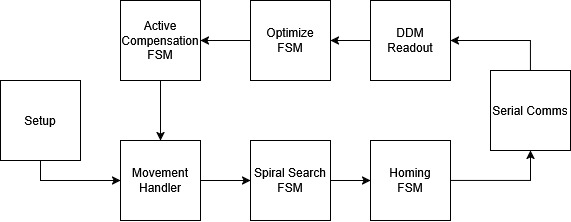
\includegraphics[width=\textwidth]{figures/STM32_flow.jpg} % Replace with your first image file
    \end{minipage}\hfill
    \begin{minipage}{0.37\textwidth}
        \centering
        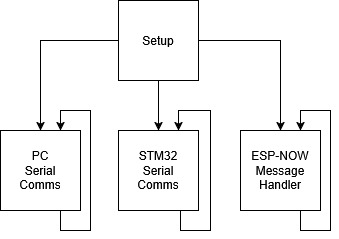
\includegraphics[width=\textwidth]{figures/ESP32_flow.jpg} % Replace with your second image file
    \end{minipage}
    \caption{Left: STM32 firmware diagram. Right: ESP32 firmware diagram}
    \label{fig9:flow_charts}
\end{figure}


\chapter{Active Alignment and Control Algorithm}
% This bridges your hardware and your [RESEARCH ASPECT]. It explains the "brain" of your system.
This chapter explains how the built platform is controlled, starting from how data is collected and then how this information is used to set up the link and keep it running.
\section{DDM Data Extraction}
% How your microcontroller communicates with the SFP module (e.g., via I2C) to constantly poll the Rx power levels.
As mentioned before, most of the modern SFP's has DDM implemented, which can be accessed by connecting to SFP's I2C pins, or using media converter functionalities.
Unfortunetely in this case, used media converter dosen't provide DDM data interface, so controler must be soldered into SFP pins.

SFP pinout is provided in the figure \ref{Fig10:sfp_pinout}. SDA is at pin 6 and SCL is at pin 5.
\begin{figure}[htbp]
  \centering
  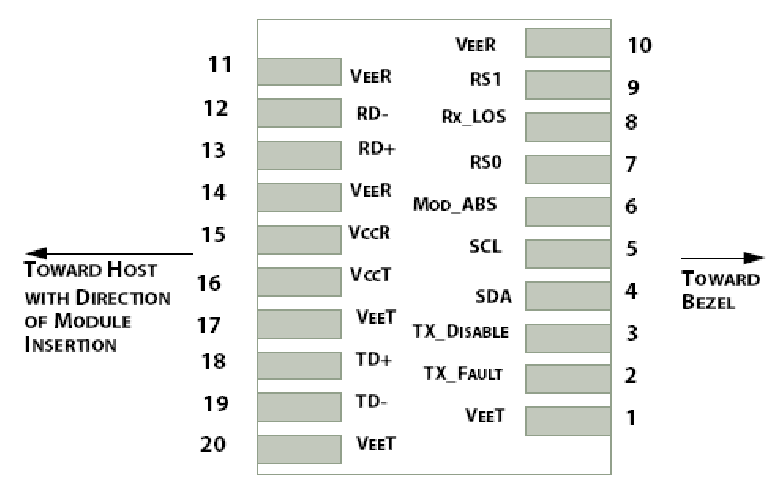
\includegraphics[width=0.85\textwidth]{figures/pinout.png}
  \caption[short]{Pinout of the sfp}
  \label{Fig10:sfp_pinout}
\end{figure}

There is a lot of different information about SFP module that can be accessed via this I2C, but the most interesting part is in "Real Time Diagnostic and Control Registers" part.
It is set of variables that are normally used to diagonse module and link health.

Specific addresses can be seen in table \ref{tab:a2h_memory_map_short}.
\begin{table}[htbp]
\centering
\renewcommand{\arraystretch}{1.2}
\begin{tabular}{|c|c|l|l|}
\hline
\textbf{A2h} & \textbf{Bit} & \multicolumn{1}{c|}{\textbf{Name}} & \multicolumn{1}{c|}{\textbf{Description}} \\ \hline
\multicolumn{4}{|l|}{\textbf{Converted analog values. Calibrated 16-bit data.}} \\ \hline
96  & All & Temperature MSB                      & Internally measured module temperature       \\ \hline
97  & All & Temperature LSB                      &                                              \\ \hline
98  & All & Vcc MSB                              & Internally measured supply voltage in transceiver \\ \hline
99  & All & Vcc LSB                              &                                              \\ \hline
100 & All & TX Bias MSB                          & Internally measured TX Bias Current          \\ \hline
101 & All & TX Bias LSB                          &                                              \\ \hline
102 & All & TX Power MSB                         & Measured TX output power                     \\ \hline
103 & All & TX Power LSB                         &                                              \\ \hline
104 & All & RX Power MSB                         & Measured RX input power                      \\ \hline
105 & All & RX Power LSB                         &                                              \\ \hline
\multicolumn{4}{|c|}{\vdots} \\ \hline
\end{tabular}
\caption{Real Time Diagnostic and Control Registers [Address A2h, Bytes 96-111] \cite{SNIASFF8472}}
\label{tab:a2h_memory_map_short}
\end{table}
\newpage
Beside this table, there is also information how to interpret those values, according to the SFF8472:
\\
"Measured RX received optical power in mW. Value can represent either average received power or OMA
depending upon how bit 3 of byte 92 (A0h) is set. Represented as a 16-bit unsigned integer with the power
defined as the full 16-bit value (0-65535) with LSB equal to 0.1 $\mu W$, yielding a total range of 0 to 6.5535 mW
(~ -40 to +8.2 dBm) \cite{SNIASFF8472}."

There is no much information about refresh rate of this data in this specification document, so that had to be checked empirically.
In case of SFP modules that were used in this transcevier, the period of updating data was $t = 15ms$, which corresponds to $f = \frac{1}{t} = \frac{1}{15 * 10^{-3}} = 66.67Hz$.

Having this information it can be concluded that with this data rate, transcevier will be capable of compensating low frequency changes.

\section{Connection Seeking Algorithm (Spiral Search)}

After placing the transceivers, so they are aimed at each other, it is though task to make them shoot perfectly "straight".
It's couse imperfections of the mechanical design, or even media converter itself, the SFP module can be a little bit rotated.
It can be calibrated it coarsely, but at the end some search algorithm had to be developed.

Applied algorithm is Square Spiral Search Pattern Method. Because the transcevier shoots almost straight, the direct neighborhood must be searched.
Flowchart has been presented in the figure \ref{Fig11:Spiral search}. The algorithm is straight forward, with asynchronous stop condition. 
Lower the dx denser the search. 
That dependency allows for using the search in different scenarios,
 like in case the connection was lost dense version will be appropiate.
During link set up rather coarse version is suggested, because the field of search is much bigger. 

\begin{figure}[htbp]
  \centering
  \includegraphics[width=0.85\textwidth]{figures/Flow_chart_spiral.jpg}
  \caption[short]{Spiral search flow chart}
  \label{Fig11:Spiral search}
\end{figure}

\section{Maximum Scan Algorithm}

During link set up, it is not required, to keep a connection. 
When a first couple milli Watts are seen on the monitoring then it's a time for Maximum Scan Algorithm.

It is algorithm that scans the given axis three times and saves maximum received power. 
During fourth and further walkthroughs it stops when it is close to the previously found maximum. 
Then it repeats the procedure for second axis.

\section{Control Algorithm Design}
%The logic used to maintain optimal beam alignment. Explain the feedback loop (e.g., PID controller, hill-climbing algorithm, or custom logic) that translates power drops into precise stepper motor steps.

When the link is already set up and used for data transfer, the continuous transmission is preferred, so a active compensation can't use same algorithm, which was used during link set up to maximize received power.
As stated in DDM section, refresh rate of received power in DDM is rather slow, the algorithm to actively compensate the changing value dosen't need to be really fast.

On top of that the power curve is rather simple with one maximum,
because we only apply the algorithm in Y and Z axis (parallel to the lens), 
since X (perpendicular to the lens) should be already well align after link set up. 
\begin{lstlisting}
  algorithm Discrete Space Hill Climbing is
    currentPow := rxPow
    previousPow := 0
    loop do
        currentPow := rxPow
        if currentPow < previousPow then
          return
        previousPow := currentPow
        move further
\end{lstlisting}


\section{Misalignment Compensation}
How the software specifically differentiates between standard signal fluctuation and physical drift caused by thermal expansion or physical transceiver head movement.


\chapter{Experimental Methodology}
% Since this is an [EXPERIMENTAL] thesis, you need to explain exactly how you tested the system.

\section{Experimental Setup}
The physical testing environment (indoor bench tests vs. outdoor free-space tests), distance of the link, and equipment used.

\section{Test Scenarios}
How you deliberately introduced misalignment to test the system (simulating thermal expansion, vibrating the mount, shifting the receiver).

\section{Measurement Metrics}
What defines "success" for your project? (e.g., Bit Error Rate (BER), packet loss, alignment recovery time, optical power stability).


\chapter{Results and Analysis}
% This is where you present your findings from the [RESEARCH ASPECT].

\section{Baseline Performance}
How the link performs statically without the active alignment control turned on.

\section{Tracking Algorithm Performance}
Graphs and data showing the system actively correcting itself when perturbed. Include response times and accuracy.

\section{Environmental Impact}
Data on how ambient conditions affected the link quality during your tests.

\section{Discussion}
An honest evaluation of your system's stability, limitations of the 3D-printed mechanics, and the speed bottleneck of polling DDM data.


\chapter{Conclusion and Future Work}

\section{Summary of Achievements}
A review of the project, confirming whether you met the objectives outlined in Chapter 1.

\section{Future Work}
What could be improved in future iterations? (e.g., faster motors, different optics, machine learning for predictive tracking).




















% \chapter{Introduction} % A chapter title
% Analog to DIgital Converters \ac{ADC} are used in a wide variety of applications...


% \chapter{Conclusion}

% Test reference to the bibliography \cite{digital_signal_processor_voigt_xu}.

\newpage

% citation format:
% [1.2] - [chapter.number of citation]
% citation for journal - J. Smith, title, journal, 2023, vol. 12, No. 10, pp-1011-1015 (possibly DOI)
% citing book - J. Smith, title, publisher, 2010, ch 8, pp...
% Citing the internet - http://... , Nov 28, 2023
% formulas:
% 123 (1) - number in brackets.

\hbadness = 10000 % Suppresses underfull hbox warnings

\bibliographystyle{plain}
\bibliography{references}
\newpage

% Appendices
\begin{appendices}

% Custom command for appendix sections
\newcommand{\appendixsection}[1]{
    \refstepcounter{section}                    % Increment the section counter
    \section*{Appendix \Alph{section}: #1}      % Format as "Appendix A: Title"
    \addcontentsline{toc}{section}{Appendix \Alph{section}: #1}% Add to TOC
}

% Do not make a new page for the first appendix
\let\clearpage\relax
\chapter{Appendices}

% First appendix: Landscape schematic
\newgeometry{left=1cm, right=1cm, top=0.5cm}
\appendixsection{ADC Board Schematic}
Nah

% First appendix: Landscape schematic
\newgeometry{left=6.0cm, right=0.5cm, top=1.0cm}
\appendixsection{DAC Board Schematic}
Nah

% Second appendix
\appendixsection{Source Code} % Continue numbering properly
\label{appendix:another} % Label for referencing

Nah

\end{appendices}

%end of the work
\end{document}
